
\subsection{Ziele von Datenbanken}
$\Rightarrow$ große Mengen an strukturierten Daten zu speichern und zu verwalten
\subsubsection*{Verwaltung (Aufgaben eines Datenbank-Management-Systems) \cite{skript}}
\begin{itemize}
    \item Festlegung von Datenstrukturen (für dauerhafte Speicherung)
    \item Mechanismen zur Manipulation von Daten
    \item Autorisierung
    \item Strategien zur Datensicherung 
\end{itemize}
Das wirkt entgegen: 
\begin{itemize}
    \item Redundanz und Inkonsistenz
    \item Umständliche Datenabfragen
    \item Probleme der \Gls{Heterogenität}
    \item Probleme der Integrität
    \item Probleme der \Gls{Atomizität}
    \item Probleme des gleichzeitigen Zugriffs
    \item Sicherheitsprobleme/Autorisierung
\end{itemize}
\subsection{Datenebenen}
\subsubsection*{Drei-Ebenen-Architektur \cite{dewiki:Datenebenen}\cite{skript}}
\begin{itemize}
    \item \textbf{physikalische Ebene (interne Ebene)}: physische Sicht der Datenbank im Computer / die Datenstrukturen mit Hilfe derer die Daten persistent (auf der Platte) gespeichert werden
    \item \textbf{logische Ebene (konzeptionelle Ebene)}: welche Daten in der Datenbank abgelegt sind und welche Beziehungen zwischen diesen bestehen
    \item \textbf{Sichten-Ebene (externe Ebene)}: Kann Benutzern und Anwendungen individuelle Benutzersichten bereitstellen
\end{itemize} 
\begin{figure}[H]
    \centering
    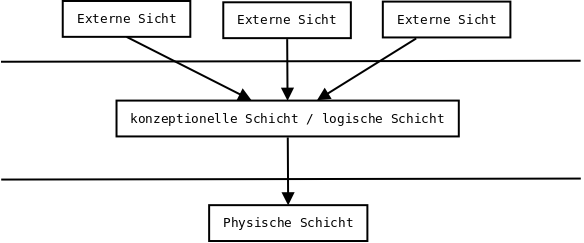
\includegraphics[width=10cm]{images/3Schichten.png}
    \caption{Visualisierung der drei Schichten eines \Glsgen{Datenbanksystem}.}
    \label{fig:3Schichten}
\end{figure} 
\begin{mybox}[title=Datenbanksystem]
Ein \Gls{Datenbanksystem} ist eine Sammlung von Daten zusammen mit einer Menge von (Software-)
Programmen, die den Zugriff und Modifikation dieser Daten erlauben und regeln.
\end{mybox}
\subsubsection*{Schemata \cite{dewiki:Schema}\cite{skript}}
\begin{itemize}
    \item Physikalisches Schema (internes Schema)
    \item Logisches Schema (konzeptionelles Schema)
    \item Schichten-Schema (externes Schema)
\end{itemize} 
\begin{mybox}[title=Schema und Instanz]
Mit \Gls{Schema} bezeichnen wir die einer Datenbank zu Grunde liegende Struktur. Wir nennen die Menge an Daten, die zu einem gegebenen Zeitpunkt in
einer Datenbank gespeichert sind, eine \Gls{Instanz} der Datenbank
\end{mybox}
\subsubsection*{Datenunabhängigkeit \cite{dewiki:Datenunabhängigkeit}\cite{skript}}
\begin{itemize}
    \item \textbf{physikalische Datenunabhängigkeit}: Änderungen im physikalischen Schema wirken sich nicht auf eine Anwendung oder das logische Schema aus
    \item \textbf{logische Datenunabhängigkeit}: Änderungen im logischen Schema wirken sich nicht auf eine Anwendung (Sicht) und somit nicht auf den Endbenutzer aus 
\end{itemize}
\subsection{Datenmodelle}
\begin{mybox}[title=Datenmodell]
Ein \Gls{Datenmodell} ist ein konzeptuelles Werkzeug, um Daten, die Beziehungen zwischen den Daten, ihre Bedeutung (Semantik) sowie Konsistenz-Bedingungen auf den Daten zu beschreiben. Das Datenmodell bestimmt die möglichen Strukturen (\Gls{Schema}) einer Datenbank.
\end{mybox}
Datenmodelle sind bspw.\cite{dewiki:Datenmodell}: 
\begin{itemize}
    \item \textbf{Konzeptuelles Datenmodell}: z.B. ER-Diagramm
    \item \textbf{Logisches Datenmodell}: z.B. relationalen Datenmodell
    \item \textbf{Physisches Datenmodell}: z.B. Indexstrukturen
\end{itemize}
\subsubsection*{Das Relationale Datenmodell \cite{skript}} \label{sec:reldatm}
Im relationalen Modell werden Daten in Form von Tabellen abgelegt. Jede Spalte entspricht einem \Gls{Attribut}.
\subsubsection*{Extensible Markup Language (XML) als Datenmodell \cite{skript}}
repräsentiert im wesentlichen Baumstrukturen. Die Beziehungen zwischen Daten werden durch Einbettung von Elementen ausgedrückt.
\subsection{Datenbanksprachen}
\subsubsection*{Data Definition Language (DDL) \cite{skript}}
 Eine \Gls{ddl} ist eine Sprache zur Spezifikation des \Glsgen{Schema} (der Struktur) und Spezifikation von Bedingungen, die jede \Gls{Instanz} der Datenbank erfüllen soll. \\
 Solche bedingungen können sein: 
 \begin{itemize}
     \item \textbf{\Glspl{Domänenbeschränkung}}: Spezifikation des gültigen Wertebereichs für ein \Gls{Attribut}
     \item \textbf{\Gls{Referentielle Integrität}}
     \item \textbf{Zugansbeschränkungen}
     \item Andere Beschränkungen: bspw. jeder Kunde, der einen Kredit besitzt, muss ein Konto mit einem Kontostand von mindestens 1.000 Euro haben
 \end{itemize}
 \subsubsection*{Data Manipulation Language (DML) \cite{skript}}
 Eine \Gls{dml} ist eine Sprache mit Mechanismen zur Abfrage, Einfügung, Änderung und Löschung von Daten. Der Teil einer \acrshort{dml}, der für die Abfrage von Daten zuständig ist, wird oft einfach \Gls{ql} genannt.
\subsection{Wichtige Begriffe und Konzepte}
\subsubsection*{Relationale Datenbanken \cite{skript}}
Relationale Datenbanken basieren auf dem relationalen Datenmodell (Abschnitt \ref{sec:reldatm}). 
\Gls{Transaktion}
%\subsubsection*{Normalisierung \cite{skript}}
%\subsubsection*{Transaktionen \cite{skript}}
%\subsection{Entwurf von Datenbanken}
\subsection{Architektur eines Datenbanksystems}
\subsection*{Web-basierte Datenbankanwendungen}

